\documentclass[12pt]{article}
\usepackage{blindtext}
\usepackage[en,bordered]{uni-style}
\usepackage{uni-math}
\usepackage{physics}
\usepackage{amssymb}
\usepackage{capt-of}
\usepackage{karnaugh-map}
\usepackage{neuralnetwork}
\usepackage{tikz}
\usepackage{graphicx,wrapfig,lipsum}
\tikzstyle{mynode}=[thick,draw=blue,fill=blue!20,circle,minimum size=22]


\usetikzlibrary{calc}

\def\layersep{3cm}
\newcommand\nn[1]{
    % Input layer
    \foreach \y in {1,...,2}
        \node[neuron, fill=green!40] (i\y-#1) at (0,\y+1) {$i\y$};

    % Hidden layer
    \foreach \y in {1,...,4}
        \path node[neuron, fill=blue!40] (h\y-#1) at (\layersep,\y) {$h\y$};

    % Output node
    \node[neuron, fill=red!40] (o-#1) at (2*\layersep,2.5) {$o$};

    % Connect every node in the input layer with every node in the hidden layer.
    \foreach \source in {1,...,2}
        \foreach \dest in {1,...,4}
            \path (i\source-#1) edge (h\dest-#1);

    % Connect every node in the hidden layer with the output layer
    \foreach \source in {1,...,4}
        \path (h\source-#1) edge (o-#1);
}

\makeatletter
\newcommand*{\rom}[1]{\expandafter\@slowromancap\romannumeral #1@}
\makeatother

\DeclareMathOperator*{\argmax}{arg\,max}
\DeclareMathOperator*{\argmin}{arg\,min}
\title{Intruduction to Machine Learning}
\prof{Dr \,S.Amini}
\subject{Homework 4}
\info{
    \begin{tabular}{lr}
        Amirreza Velae & 400102222\\
        github    & \href{https://github.com/amirrezavelae}{repository}\\
    \end{tabular}
    }
    \date{\today}
    % \usepackage{xepersian}
    % \settextfont{Yas}
    \usepackage{uni-code}
    
\begin{document}
\maketitlepage
\maketitlestart

\section{Representer Theorem}
In your own words, explain the meaning of each term below (you don’t need to get too technical here. The aim is to ensure that you have enough knowledge to answer the next part. Don’t freak out!):
\begin{itemize}
    \item Hilbert Space
    \item Reproducing Kernel Hilbert Space
    \item Reproducing Kernel
    \item Mercer’s Theorem
\end{itemize}

\begin{qsolve}[Hilbert Space]
    Hilbert space is a generalization of Euclidean vector spaces on witch we define inner product.
    \\ An inner product on a complex linear space $\mathcal{X}$ is defined as:
    \begin{gather*}
        (. , .) : X \cross X \rightarrow \mathbb{C}
    \end{gather*}
    Such that, for all $x,y.z \in \mathcal{X}$ and $\lambda  , \mu \in \mathbb{C}$:
    \begin{itemize}
        \item $(x,\lambda y + \mu z) = \lambda(x,y) + \mu(x,z)$ (Linearity)
        \item $(x,y) = (y,x)$ ( Hermitian symmetric)
        \item $(x,x)\geq 0$(Nonnegative)
        \item $(x,x) =0 $ iff $x=0$ (PD)
    \end{itemize}
    We call a linear space with an inner product an \textit{inner product space} or \textit{pre-Hilbert space}.
    \\Banach space is a complete normed vector space. Thus, a Banach space is a vector space with a metric that allows the computation of vector length and distance between vectors and is complete in the sense that a Cauchy sequence of vectors always converges to a well-defined limit that is within the space.
    if $\mathcal{X}$ is a linear space with an inner product $(. , .)$, then we can define a norm on $\mathcal{X}$ by
    \begin{gather*}
        \norm*{x} = \sqrt{(x,x)}
    \end{gather*}
    \splitqsolve
    A Hilbert Space is an inner product space that is complete and separable with respect to the
    norm defined by the inner product i.e. every Hilbert space is a Banach space with respect to the norm in it.
\end{qsolve}


\begin{qsolve}[Reproducing Kernel Hilbert Space]
    A Reproducing Kernel Hilbert Space (RKHS) is a Hilbert space H with a reproducing kernel whose span
    is dense in H. We could equivalently define an RKHS as a Hilbert space of functions with all evaluation
    functionals bounded and linear.
    \\For a (compact) $\mathcal{X} \subseteq \mathbb{R}^d$, and a Hilbert space $\mathcal{H}$ of functions $f:\mathcal{X} \rightarrow \mathbb{R}$, we say $\mathcal{H}$ is a \textit{Reproducing Kernel Hilbert Space} if $\exists k : \mathcal{X} \rightarrow \mathbb{R}$,s.t.
    \begin{itemize}
        \item  $k$ has the reproducing property, i.e., $f(x) = \left\langle  f(.),k(.,x) \right\rangle $
        \item  $k$ spans $\mathcal{H} = \overline{span\{k(.,x):x \in \mathcal{X}\}}$
    \end{itemize}
\end{qsolve}

\begin{qsolve}[Reproducing Kernel]
    A reproducing kernel of a Hilbert space $\mathcal{H}$ is a function $k:\mathcal{X} \cross \mathcal{X} \rightarrow \mathbb{R}$ such that
    \begin{itemize}
        \item $k$ is symmetric, i.e., $k(x,y) = k(y,x)$
        \item $k$ is positive semi-definite, i.e., $\forall n \in \mathbb{N}, \forall x_1,...,x_n \in \mathcal{X}, \forall c_1,...,c_n \in \mathbb{R}$
              \begin{gather*}
                  \sum_{i=1}^{n} \sum_{j=1}^{n} c_i c_j k(x_i,x_j) \geq 0
              \end{gather*}
        \item $k$ has the reproducing property, i.e., $\forall x \in \mathcal{X}, \forall f \in \mathcal{H}$
              \begin{gather*}
                  f(x) = \left\langle  f(.),k(.,x) \right\rangle
              \end{gather*}
    \end{itemize}
\end{qsolve}

\begin{qsolve}[Mercer’s Theorem]
    Let $\mathcal{X}$ be a compact set and $k:\mathcal{X} \cross \mathcal{X} \rightarrow \mathbb{R}$ be a continuous symmetric positive semi-definite function. Then, there exists a Hilbert space $\mathcal{H}$ and a function $\phi:\mathcal{X} \rightarrow \mathcal{H}$ such that
    \begin{gather*}
        k(x,y) = \left\langle  \phi(x),\phi(y) \right\rangle
    \end{gather*}
\end{qsolve}

\textbf{Theorem 1.1.} (Representer Theorem). Consider The following optimization problem:
\begin{gather*}
    f^* = \argmin_{f \in \mathcal{H}_{\mathcal{K}}} \mathcal{L} (f) \\
    \mathcal{L}_{\mathcal{K}} = \frac{1}{N} \sum_{i=1}^{N} l(y_i , f(x_i)) + R(\norm*{f})
\end{gather*}
where $\mathcal{L}_{\mathcal{K}}$ is an RKHS with kernel $\mathcal{K}$, $l(y,\hat{y})\in R$ is a loss function, and $R(c) \in R$ is a strictly monotonicly increasing penalty function, and
\begin{gather*}
    \norm*{f}_{\mathcal{H}} = \sqrt{{\left\langle  f,f \right\rangle}_{\mathcal{H}}}
\end{gather*}
is the norm of the function. Then we have
\begin{gather}
    f^*(x) = \sum_{k=1}^{N} \alpha_k \mathcal{K}(x,x_k)
\end{gather}
where $\alpha_k \in R$ are the coefficients depend on the training data$\{(x_i,y_i)\}$
\\ \textbf{Important: For each of the questions below, explain and motivate your answers!}
\\Use the Mercer’s theorem to write $f \in \mathcal{H}_{\mathcal{K}}$ in the following form:
\begin{gather*}
    f(x_j) =\sum_{k=1}^{N} \alpha_k \Phi(x_k) +v(x_j)
\end{gather*}
where $\Phi_k(.)$ and $v(.)$ are orthogonal i,e, $\left\langle  \Phi(.),v(.) \right\rangle = 0$
\begin{qsolve}
    \begin{gather*}
        f^*(x) = \sum_{k=1}^{N} \alpha_k \mathcal{K}(x,x_k) \\
        \mathcal{K}(x,x_k) = \left\langle  \Phi(x),\Phi(x_k) \right\rangle \\
        f^*(x) = \sum_{k=1}^{N} \alpha_k \left\langle  \Phi(x),\Phi(x_k) \right\rangle \\
        f^*(x) = \sum_{k=1}^{N} \alpha_k \Phi(x) \Phi(x_k) \\
    \end{gather*}
\end{qsolve}

\clearpage
\section{Neural Networks Can be Seen as (almost) GPs!}
In this problem, we explore an interesting property of Gaussian processs:
\subsection{2.1}
Consider an MLP with one hidden layer and activation functions $h_j(x), j = 1, . . . , H$:
\begin{gather*}
    f_k(x) = b_k + \sum_{j=1}^{H} v_{jk} h_j(x) \\
    h_j(x) = h(u_{0j} + x^T u_j) \\
\end{gather*}
where H is the number of hidden units, and $h()$ is some nonlinear activation function, such
as the ReLU. Assume Gaussian prior on the parameters (each set of parameters below are
independent from the other sets):
\begin{gather*}
    b_k \sim \mathcal{N}(0,\sigma_b^2) \\
    v_{jk} \sim \mathcal{N}(0,\sigma_v^2) \\
    u_{0j} \sim \mathcal{N}(0,\sigma_{u_0}^2) \\
    u_j \sim \mathcal{N}(0,\sigma_u^2) \\
\end{gather*}
Denote all the parameters by $\theta$.
\subsubsection{2.1.1}
Show that the expected output of the network is 0, i.e., $\mathbb{E}_\theta[f_k(x)] = 0$.
\begin{qsolve}
    \begin{gather*}
        f_k(x) = b_k + \sum_{j=1}^{H} v_{jk} h_j(x) \\
        h_j(x) = h(u_{0j} + x^T u_j) \\
        \mathbb{E}[f_k(x)] = \mathbb{E}[b_k] + \sum_{j=1}^{H} \mathbb{E}[v_{jk}] \mathbb{E}[h_j(x)] \\
        \mathbb{E}[f_k(x)] = 0 + \sum_{j=1}^{H} 0 \mathbb{E}[h_j(x)] \\
        \mathbb{E}[f_k(x)] = 0 \\
    \end{gather*}
\end{qsolve}
\subsubsection{2.1.2}
Show that the covariance of the output for two different inputs is the following:
\begin{gather*}
    \mathbb{E}_\theta[f_k(x)f_k(x')] = \sigma_b^2 + \sigma_v^2 H \mathbb{E}[h_j(x)h_j(x')]
\end{gather*}
\begin{qsolve}
    \begin{gather*}
        \mathbb{E}[f_k(x)f_k(x')] = \mathbb{E}[(b_k + \sum_{j=1}^{H} v_{jk} h_j(x))(b_k + \sum_{j=1}^{H} v_{jk} h_j(x'))] \\
        \mathbb{E}[f_k(x)f_k(x')] = \mathbb{E}[b_k^2 + \sum_{j=1}^{H} v_{jk}^2 h_j(x) h_j(x') + b_k \sum_{j=1}^{H} v_{jk} h_j(x') + b_k \sum_{j=1}^{H} v_{jk} h_j(x)] \\
        = \mathbb{E}[b_k^2] + \sum_{j=1}^{H} \mathbb{E}[v_{jk}^2] \mathbb{E}[h_j(x) h_j(x')] + \mathbb{E}[b_k] \sum_{j=1}^{H} \mathbb{E}[v_{jk}] \mathbb{E}[h_j(x')] + \mathbb{E}[b_k] \sum_{j=1}^{H} \mathbb{E}[v_{jk}] \mathbb{E}[h_j(x)] \\
        \mathbb{E}[f_k(x)f_k(x')] = \sigma_b^2 + \sum_{j=1}^{H} \sigma_v^2 \mathbb{E}[h_j(x) h_j(x')] + 0 + 0 \\
        \mathbb{E}[f_k(x)f_k(x')] = \sigma_b^2 + \sum_{j=1}^{H} \sigma_v^2 \mathbb{E}[h_j(x) h_j(x')] \\
        \mathbb{E}[f_k(x)f_k(x')] = \sigma_b^2 + H \sigma_v^2 \mathbb{E}[h_j(x) h_j(x')] \\
    \end{gather*}
\end{qsolve}
\subsubsection{2.1.3}
Using the central limit theorem, argue that as $H \rightarrow \infty$, the output of the network converges
to a multivariate Gaussian distribution with mean and covariance calculated above. This is
equivalent to a Gaussian process (this kernel can be computed in close form for certain activation
functions such as the ReLU.)
\begin{qsolve}
    CLT states that the sum of a large number of independent random variables, each with finite mean and variance, will be approximately normally distributed. \\
    As $H \rightarrow \infty$, we have:
    \begin{gather*}
        \sigma_{\bar{f}}^2 = \frac{\sigma_b^2}{H} + \sigma_v^2 \mathbb{E}[h_j(x) h_j(x')] \\
        H \rightarrow \infty \Rightarrow \sigma_{\bar{f}}^2 = \sigma_v^2 \mathbb{E}[h_j(x) h_j(x')] \\
        \mu_{\bar{f}} = 0 \\
    \end{gather*}
\end{qsolve}

\subsection{2.2}
The result above can also be extended to arbitrary deep neural networks. Search ”Neural
tangent kernels” and in two paragraphs, explain your understanding of what they are (Note:
it’s not necessarily practical to always use GPs instead of neural networks).
\begin{qsolve}
    Neural tangent kernels are a way to approximate the output of a neural network with a Gaussian process. \\
    The idea is to use the neural network as a feature extractor and then use the features as inputs to a Gaussian process. \\
    The neural tangent kernel is the covariance function of the Gaussian process. \\
    The neural tangent kernel is defined as:
    \begin{gather*}
        k(x, x') = \mathbb{E}_{\theta \sim \mathcal{N}(0, I)}[f(x, \theta) f(x', \theta)] \\
    \end{gather*}
    where $f(x, \theta)$ is the output of the neural network with input $x$ and parameters $\theta$. \\
    The neural tangent kernel is a function of the input data $x$ and $x'$ and is independent of the parameters $\theta$. \\
\end{qsolve}

\section{SVM}
\subsection{3.1}
In the soft-margin SVM problem, the slack value $\xi_i$ takes three possible values for the ith
sample: ($\xi_i = 0$, $0 < \xi_i \leq 1$, $1 < \xi_i$). For each of these scenarios, where does the point lie relative
to the margin? Is the point classified correctly?
\begin{qsolve}
    \begin{itemize}
        \item $\xi_i = 0$: The point lies on the margin.
        \item $0 < \xi_i \leq 1$: The point lies inside the margin.
        \item $1 < \xi_i$: The point lies on the wrong side of the margin.
    \end{itemize}
\end{qsolve}

\subsection{3.2}
Each of the datasets below contains points beloning to two classes $\{-1, 1\}$(positives and negatives correspond to 1 and -1). For each dataset, find a transformation of the features $\mathbf{X}_1$ and $\mathbf{X}_2$
such that the points are linearly separable (can be separated by a line in the new expanded
feature space).
\begin{figure}[h]
    \centering
    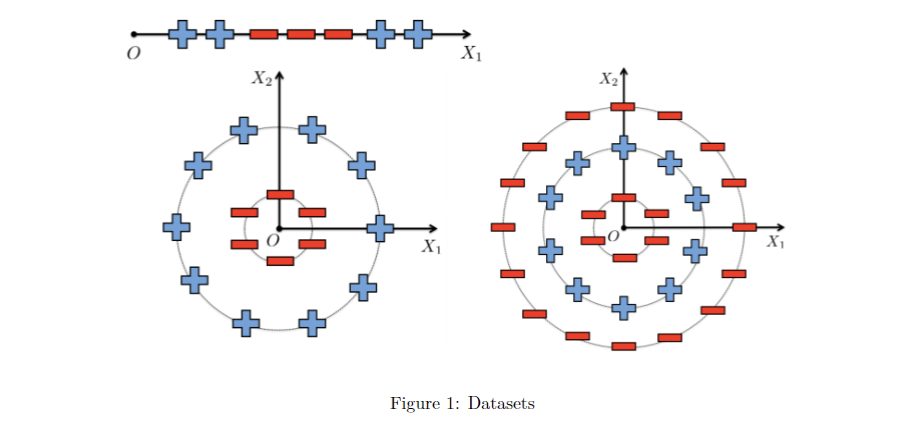
\includegraphics[width=0.75\textwidth]{Q3.png}
\end{figure}

\begin{qsolve}
    \begin{itemize}
        \item Dataset 1: $\lvert \mathbf{X}_1 - \bar{\mathbf{X}}_1 \rvert \geq \alpha$
        \item Dataset 2: $\mathbf{X}_1^2 + \mathbf{X}_2^2 \geq \alpha$
        \item Dataset 3: $-1 \times (\alpha \leq \mathbf{X}_1^2 + \mathbf{X}_2^2 \leq \beta)$
    \end{itemize}
\end{qsolve}

\section{Interpretation Via Maximum Projection Spread}
In this point of view we need some directions that have maximum data projection variance.
Derive sample covariance matrix and show that the linear projection onto an M -dimensional
subspace that maximizes the variance of the projected data is defined by the M eigenvectors of
the sample covariance matrix S, corresponding to the M largest eigenvalues.

\begin{qsolve}[Interpretation Via Maximum Projection Spread]
    \begin{gather*}
        \mathbb{X} = \begin{bmatrix}
            \mathbf{x}_1^T \\
            \mathbf{x}_2^T \\
            \vdots         \\
            \mathbf{x}_n^T \\
        \end{bmatrix} \\
        \mathbf{E}_D [x] = \frac{1}{n} \sum_{i=1}^n \mathbf{x}_i =\bar{x}\\
        Cov[x] = \frac{1}{n} \sum_{i=1}^n (\mathbf{x}_i - \bar{x})(\mathbf{x}_i - \bar{x})^T = S \\
        \bar{x} = \frac{1}{N} \mathbb{X}^T \mathbf{1} \\
        S = \frac{1}{N} \mathbb{X}^T \mathbb{X} - \bar{x} \bar{x}^T = \frac{1}{N} \mathbb{X}^T \mathbb{X} - \frac{1}{N^2} \mathbb{X}^T \mathbf{1} \mathbf{1}^T \mathbb{X} = \frac{1}{N} \mathbb{X}^T (\mathbf{I} - \frac{1}{N} \mathbf{1} \mathbf{1}^T) \mathbb{X} \\
    \end{gather*}
    If we assume $\mathbf{H} = (\mathbf{I} - \frac{1}{N} \mathbf{1} \mathbf{1}^T)$where $\mathbf{H}$ is a projection matrix. then we have:
    \begin{gather*}
        S = \frac{1}{N} \mathbb{X}^T \mathbf{H} \mathbb{X} \\
    \end{gather*}
    Now we want to find the maximum variance of the projected data, which is $\mathbf{w}^T S \mathbf{w} $.\\
    So we have this optimization problem:
    \begin{gather*}
        \max_{\mathbf{w}} \mathbf{w}^T S \mathbf{w} \\
        s.t. \mathbf{w}^T \mathbf{w} = 1 \\
    \end{gather*}
    \splitqsolve
    If we decompose $S$ into $S = \mathbf{U} \mathbf{\Lambda} \mathbf{U}^T$ where $\mathbf{U}$ is the eigenvector matrix and $\mathbf{\Lambda}$ is the eigenvalue matrix. Then, define a new vector $\mathbf{y} = \mathbf{U}^T \mathbf{w}$, we have:
    \begin{gather*}
        \max_{\mathbf{y}} \mathbf{y}^T \mathbf{\Lambda} \mathbf{y} \\
        s.t. \mathbf{y}^T \mathbf{y} = 1 \\
    \end{gather*}
    Since $\mathbf{\Lambda}$ is a diagonal matrix, we can see that the maximum value of $\mathbf{y}^T \mathbf{\Lambda} \mathbf{y}$ is the largest eigenvalue of $\mathbf{\Lambda}$, which is the largest eigenvalue of $S$. Thus the maximum variance of the projected data is the largest eigenvalue of $S$.\\
    Also $\mathbf{w}$ is the eigenvector corresponding to the largest eigenvalue of $S$.
\end{qsolve}

\section{Interpretation Via Reconstruction}
Prove the following statement:
\begin{gather*}
    \norm*{x_i - \sum_{j=1}^{k}z_{ij}v_j}^2 = x_{i}^T x_{i} - \sum_{j=1}^{k}v_{j}^T x_{i} x_{i}^T v_{j} \\
\end{gather*}
\begin{qsolve}[Interpretation Via Reconstruction]
    \begin{gather*}
        \norm*{x_i - \sum_{j=1}^{k}z_{ij}v_j}^2 = (x_i - \sum_{j=1}^{k}z_{ij}v_j)^T (x_i - \sum_{j=1}^{k}z_{ij}v_j) \\
        = x_i^T x_i - x_i^T \sum_{j=1}^{k}z_{ij}v_j - \sum_{j=1}^{k}z_{ij}v_j^T x_i + \sum_{j=1}^{k}z_{ij}v_j^T \sum_{j=1}^{k}z_{ij}v_j \\
        = x_i^T x_i - 2 \sum_{j=1}^{k}z_{ij}v_j^T x_i + \sum_{j=1}^{k}z_{ij}^2 v_j^T v_j \\
        = x_i^T x_i - 2 \sum_{j=1}^{k}z_{ij}v_j^T x_i + \sum_{j=1}^{k}z_{ij}^2 \\
    \end{gather*}
    If take the derivate of $z_{ij}$, we have:
    \begin{gather*}
        \frac{\partial}{\partial z_{ij}} \norm*{x_i - \sum_{j=1}^{k}z_{ij}v_j}^2 = -2 v_j^T x_i + 2 z_{ij} \\
    \end{gather*}
    \splitqsolve
    Let the derivative be zero, we have:
    \begin{gather*}
        z_{ij} = v_j^T x_i \\
    \end{gather*}
    Then we can plug $z_{ij}$ back to the original equation:
    \begin{gather*}
        \norm*{x_i - \sum_{j=1}^{k}z_{ij}v_j}^2 = x_{i}^T x_{i} - \sum_{j=1}^{k}v_{j}^T x_{i} x_{i}^T v_{j} \\
    \end{gather*}
    Loss function defines as:
    \begin{gather*}
        L = \sum_{i=1}^{n} \norm*{x_i - \sum_{j=1}^{k}z_{ij}v_j}^2        = \sum_{i=1}^{n} (x_{i}^T x_{i} - \sum_{j=1}^{k}v_{j}^T x_{i} x_{i}^T v_{j}) = const - v^T S v\\
    \end{gather*}
    where $S = \frac{1}{n} \sum_{i=1}^{n} x_{i} x_{i}^T$ is the covariance matrix.\\
    Thus, the optimization problem is:
    \begin{gather*}
        \max_{v} v^T S v \\
        s.t. v^T v = 1 \\
    \end{gather*}
    which is the same as the previous problem.
\end{qsolve}

\section{Whitening Using PCA}
Whitening is one of the pre-processing techniques which is used in practical ML. By whitening,
we mean that for a given feature matrix X, this feature matrix should have zero mean vector
and identity matrix as its covariance matrix. Explain that how we could transform X by using
its covariance matrix principal components in order to have a whitened data set? After that,
prove this new feature matrix has the desired properties, namely, zero mean vector and identity
matrix as its covariance matrix.
\begin{qsolve}[Whitening Using PCA]
    To whiten the data, we need to transform the data into a new space where the mean is zero and the covariance matrix is identity matrix.\\
    First, we need to calculate the mean and covariance matrix of the data:
    \begin{gather*}
        \mu = \frac{1}{n} \sum_{i=1}^{n} x_{i} \; \; \; \; \& \; \; \; \;
        S = \frac{1}{n} \sum_{i=1}^{n} x_{i} x_{i}^T \\
    \end{gather*}
    \splitqsolve
    Then, we need to find the eigenvectors and eigenvalues of the covariance matrix $S$.\\
    Let $S = \mathbf{U} \mathbf{\Lambda} \mathbf{U}^T$, where $\mathbf{U}$ is the eigenvector matrix and $\mathbf{\Lambda}$ is the eigenvalue matrix.\\
    Then, we can transform the data into the new space by:
    \begin{gather*}
        \mathbf{y} = \mathbf{\Lambda}^{-\frac{1}{2}} \mathbf{U}^T (\mathbf{x} - \mu) \\
    \end{gather*}
    where $\mathbf{\Lambda}$ is the eigenvalue vector.\\
    The mean of the new data is:
    \begin{gather*}
        \bar{\mathbf{y}} = \frac{1}{n} \sum_{i=1}^{n} \mathbf{y}_{i} = \frac{1}{n} \sum_{i=1}^{n} \mathbf{\Lambda}^{-\frac{1}{2}} \mathbf{U}^T (\mathbf{x}_{i} - \mu) = \mathbf{\Lambda}^{-\frac{1}{2}} \mathbf{U}^T (\frac{1}{n} \sum_{i=1}^{n} \mathbf{x}_{i} - \mu) = \mathbf{\Lambda}^{-\frac{1}{2}} \mathbf{U}^T (\mu - \mu) = \mathbf{0} \\
    \end{gather*}
    The covariance matrix of the new data is:
    \begin{gather*}
        S_{y} = \frac{1}{n} \sum_{i=1}^{n} \mathbf{y}_{i} \mathbf{y}_{i}^T = \frac{1}{n} \sum_{i=1}^{n} \mathbf{\Lambda}^{-\frac{1}{2}} \mathbf{U}^T (\mathbf{x}_{i} - \mu) (\mathbf{x}_{i} - \mu)^T \mathbf{U} \mathbf{\Lambda}^{-\frac{1}{2}} \\
        = \mathbf{\Lambda}^{-\frac{1}{2}} \mathbf{U}^T (\frac{1}{n} \sum_{i=1}^{n} (\mathbf{x}_{i} - \mu) (\mathbf{x}_{i} - \mu)^T) \mathbf{U} \mathbf{\Lambda}^{-\frac{1}{2}} = \mathbf{\Lambda}^{-\frac{1}{2}} \mathbf{U}^T S \mathbf{U} \mathbf{\Lambda}^{-\frac{1}{2}} \\
        = \mathbf{\Lambda}^{-\frac{1}{2}} \mathbf{U}^T \mathbf{U} \mathbf{\Lambda} \mathbf{U}^T \mathbf{U} \mathbf{\Lambda}^{-\frac{1}{2}} = \mathbf{\Lambda}^{-\frac{1}{2}} \mathbf{\Lambda} \mathbf{\Lambda}^{-\frac{1}{2}} = \mathbf{I} \\
    \end{gather*}
\end{qsolve}

\section{Principal Components with Missing Values}
Suppose that some of the observations $x_{ij}$ of the data matrix $X$ are missing. Suggest an
algorithm that can both impute the missing values and find the principal component at the
same time.
\begin{qsolve}[Principal Components with Missing Values]
    One way to use PCA to impute missing data is to assume that the data follows a multivariate normal distribution, and that the missing values are missing at random. This means that the probability of a value being missing does not depend on its value or any other variable. Under this assumption, you can estimate the mean and covariance matrix of the data using the available values, and then use them to compute the principal components. Then, you can project the data onto the principal components, and use the inverse transformation to fill in the missing values with their expected values based on the mean and covariance matrix.\\
    \splitqsolve
    The first step is identical to the pairwise correlation (PairCor) procedure as discussed by Dray and Josse (2015), with the extension that centered PCA starting from covariances (PairCov) may also be performed via the same algorithmic steps. Essentially, either function is computed for each pair of variables based on observations for which the values of both variables are known. The correlation for variables i and h is given by
    \begin{gather*}
        r_{ih} = \frac{\sum_{j=1}^{n} (x_{ij} - \bar{x}_{i})(x_{jh} - \bar{x}_{h})}{\sqrt{\sum_{j=1}^{n} (x_{ij} - \bar{x}_{i})^2} \sqrt{\sum_{j=1}^{n} (x_{jh} - \bar{x}_{h})^2}} \\
    \end{gather*}
    where $\bar{x}_{i}$ and $\bar{x}_{h}$ are the means of variables i and h, respectively. The covariance for variables i and h is given by
    \begin{gather*}
        s_{ih} = \frac{\sum_{j=1}^{n} (x_{ij} - \bar{x}_{i})(x_{jh} - \bar{x}_{h})}{n} \\
    \end{gather*}
    we can use the correlation matrix or the covariance matrix to perform PCA.
    \\
    \href{https://www.sciencedirect.com/science/article/pii/S1574954121000261}{Source}
\end{qsolve}
\section{Clustering}
\subsection{8.1}
In each sample below, draw the boundry that K-means finds for $K = 2$. Do you think the
clusters separated by borders found by K means is meaningfull in each case? If not, what
property of data causes this?(*Recommend some solutions for these problems)
\begin{figure}[h]
    \centering
    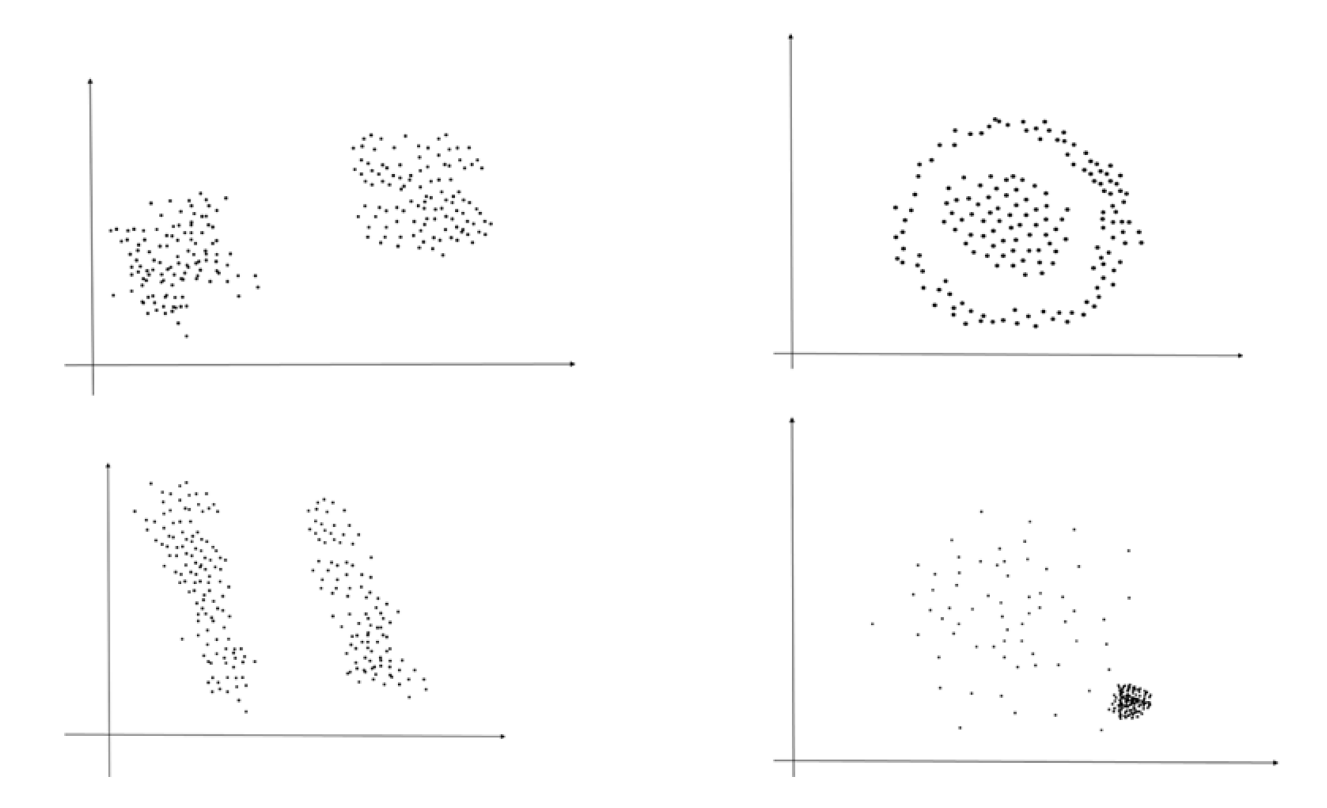
\includegraphics[width=0.8\textwidth]{Q8.png}
    \caption{8.1}
    \label{fig:8.1}
\end{figure}
\begin{qsolve}[Clustering]
    If the data is not linearly separable, then the clusters separated by borders found by K means is not meaningful.\\
    So probably, results of K-means clustering are not meaningful in (b) and (d).\\
    \begin{center}
        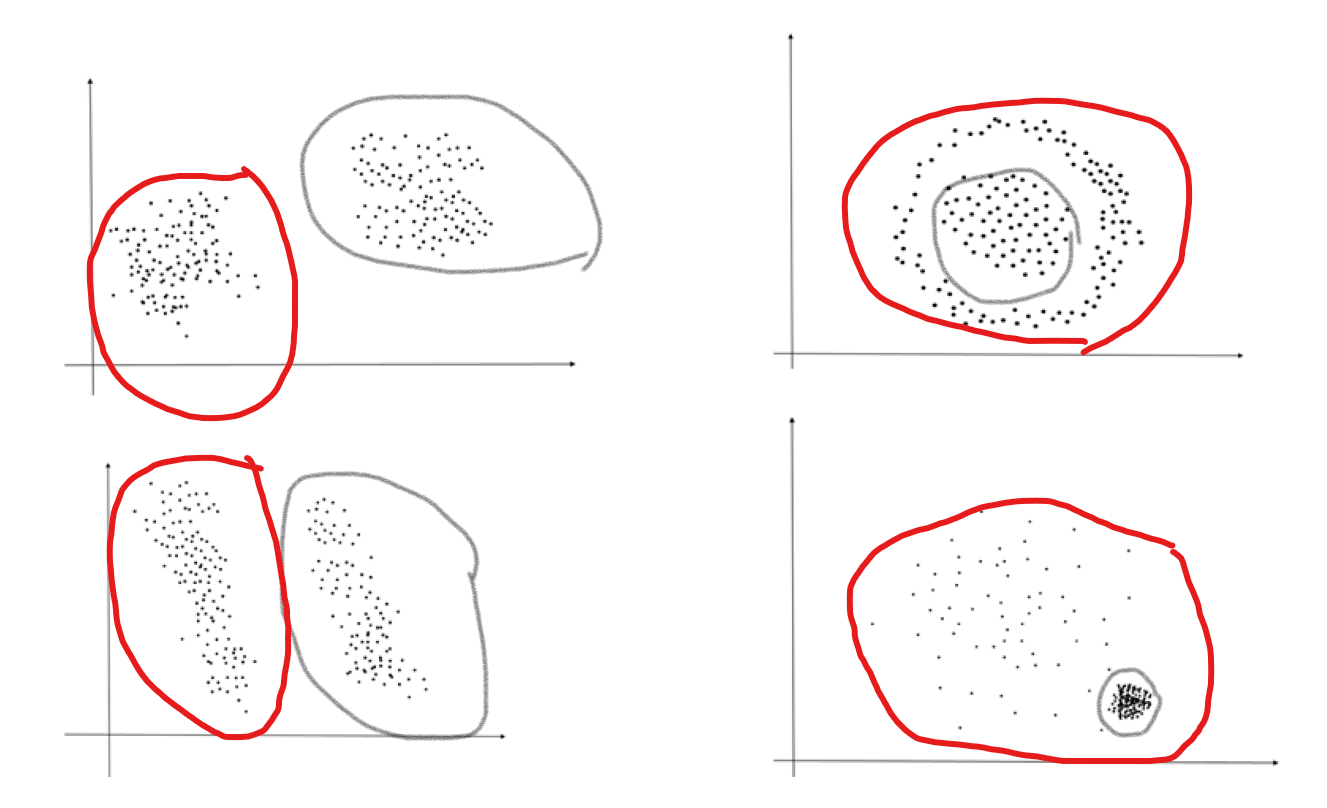
\includegraphics[width=0.8\textwidth]{Q8_solution.png}
    \end{center}
    As its clear, Data in (a) and (c) are linearly separable, so K-means clustering is meaningful in these cases.But in (b), data is not linearly separable, i.e they have same mean but different variance. So K-means clustering is not meaningful in this case; also in (d), data is not linearly separable, i.e they have different mean and different variance, but they are not linearly separable. So K-means clustering is not meaningful in this case too.\\
\end{qsolve}

\subsection{8.2}
Is it important to choose initiall points carfully in Kmeans clustering?
Illustrate it with some examples.(You can use examples above)
\begin{qsolve}[Clustering]
    Yes, it is important to choose initial points carefully in Kmeans clustering.    For example, if we choose initial points in (a) and (b) as shown in the figure below, we will get different results.\\
    \begin{wrapfigure}{l}{0.3\textwidth}
        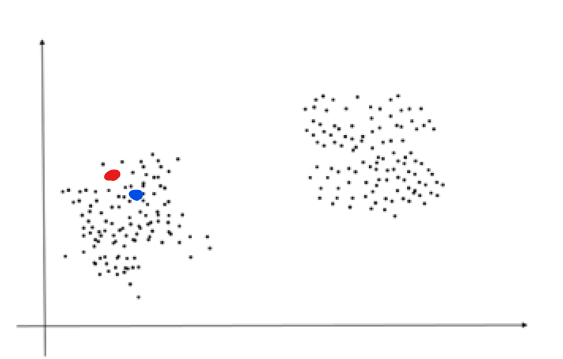
\includegraphics[width=0.24\textwidth]{Q8_solution2.png}
        \centering
    \end{wrapfigure}
    As its clear, if we choose initial points in (a) where they are far from each other, we will get better results than choosing initial points which are close to each other. Also in (b), if we choose initial points in the middle of the data, we will get better results than choosing initial points which are far from the data.\\
\end{qsolve}
\subsection{8.3}
Now you have found that initializing the points randomly is not always good. Because of that we should assign initiall points more carefully.\\
Explain \textit{Kmeans++} algorithm and define WCSS and elbow method.
\begin{qsolve}[Clustering]
    \begin{itemize}
        \item \textbf{Kmeans++} is an algorithm for choosing the initial values (or "seeds") for the k-means clustering algorithm. It was proposed in 2007 by David Arthur and Sergei Vassilvitskii, as an approximation algorithm for the NP-hard k-means problem—a way of avoiding the sometimes poor clusterings found by the standard k-means algorithm. It is similar to the first of three seeding methods proposed in 2003 by Charles Elkan, which he called k-means$||$. In this approach, the first cluster is chosen uniformly at random from the data points that are being clustered, after which each subsequent cluster is chosen from the remaining data points with probability proportional to its squared distance from the point's closest existing cluster. Repeating this procedure yields the final clustering.\\
        \item \textbf{WCSS} is the sum of squared distances between each point and the centroid in a cluster. The goal is to minimize the sum. When we plot the WCSS with the number of clusters, the plot looks like an arm. The idea of the elbow method is to identify the value of k where the distortion begins to increase most rapidly, which will become clearer when we look at an example.\\
        \item \textbf{Elbow method} is a method of interpretation and validation of consistency within cluster analysis designed to help finding the appropriate number of clusters in a dataset. In this method, we plot a line chart of the WCSS for a range of values of k (number of clusters). As the number of clusters increases, the WCSS value will start to decrease. At some point, the WCSS value will start to level off. The point where the line chart looks like an arm is called the elbow, and it marks the optimal value of k.\\
    \end{itemize}
\end{qsolve}















\makeendpage
\end{document}